%!TEX root = ../thesis.tex
%*******************************************************************************
%****************************** Second Chapter *********************************
%*******************************************************************************

\chapter{LITERATURE REVIEW}

\ifpdf
    \graphicspath{{Chapter2/Figs/Raster/}{Chapter2/Figs/PDF/}{Chapter2/Figs/}}
\else
    \graphicspath{{Chapter2/Figs/Vector/}{Chapter2/Figs/}}
\fi

Awali pembahasan pada bab ini dengan mengutarakan Problem pada Problem Domain dari tesis. Setelah itu, penjelasan tersebut diiringi dengan teori-teori penunjang pada bidang  pengetahuan yang terkait dengan Problem Domain dan Problem. Untuk lebih menguatkan klaim orisinalitas tesis penulis, perlu diberikan ulasan tentang penelitian-penelitian terkait yang juga bertujuan untuk mencoba menyelesaikan Problem tersebut. 

\section{Supporting Theory}
Uraikan dengan jelas dasar teori yang menunjang penelitian tesis yang akan dilakukan. Teori penunjang menguraikan dasar-dasar teori, temuan, dan bahan  dari pustaka ilmiah lain, yang dijadikan landasan untuk melakukan tesis yang diusulkan. Uraian dalam Teori Penunjang menjadi landasan untuk menyusun kerangka atau konsep yang akan digunakan dalam tesis.
\subsection{Augmented Intelligence in Industry 4.0}
The concept of Augmented Intelligence (AuI) is designed to improve human intelligence and help humans work to be smarter and faster. AuI includes understanding, reasoning, learning, and assurance that benefits both parties \cite{Wojcik2020}. AuI is now widely used to increase productivity, and save human time, and organizational funds by providing predictions, improving decision making, and responding to service user needs. The advantage of using AuI is that it can provide predictions using historical data. In this case, feedback is needed to improve the algorithm and to ensure it runs as expected. The application of AuI is not about replacing humans but rather finding a way that facilitates humans on a large scale with the intervention of human instincts. This means that artificial intelligence alone will not work, it is human intelligence that is at the center of innovation.

\section{Related Work}
Penelitian terkait memuat hasil penelitian pihak lain yang mempunyai Problem yang sama dengan penelitian kita, tetapi dengan menggunakan Uniqueness yang berbeda. Disini ceritakan bagaimana penelitian-penelitian terkait telah mencoba untuk menyelesaikan permasalahan yang sama dengan kita, dengan cara mereka masing-masing yang ditunjukkan dengan kutipan terhadap pustaka. Penelitian terkait yang baik melibatkan kajian pustaka yang relevan dan terpercaya dari jurnal ilmiah internasional ataupun nasional, presentasi ilmiah internasional ataupun nasional, dan buku atau catatan rujukan ilmiah. Penulis harus mencantumkan sumber referensi pada daftar pustaka manakala penulis melakukan rujukan dan kutipan dari pihak lain secara jujur dan benar seperti ini \citep{Hwang2016}.

\subsection{Effects of An Augmented Reality-based Educational Game on Students
Learning Achievements and Attitudes in RealWorld Observations}
Research conducted by Gwo Jen Hwang et al. namely creating an AR-based learning platform with a game approach to support teaching and learning activities in the real world \citep{Hwang2016}. This experiment was tested on elementary school students to explore the surrounding environment while doing recreational field trips. The AR structure in Figure \ref{fig:my_label}. developed consists of a game UI, a learning management mechanism, a learning guide mechanism, and a game mechanism. some data is stored in a database containing student profiles, learning portfolio databases, mini-games databases, and learning materials databases. The main difference between the proposed game and the traditional board game is that the game's players need to move around the real-world environment and find answers to in-game questions by making observations in the real-world environment. They need to face some of the direct challenges presented through AR technology. In this study, the teacher provides game content and manages accounts to provide question scenarios to students.

\begin{figure}[h!]
    \centering
    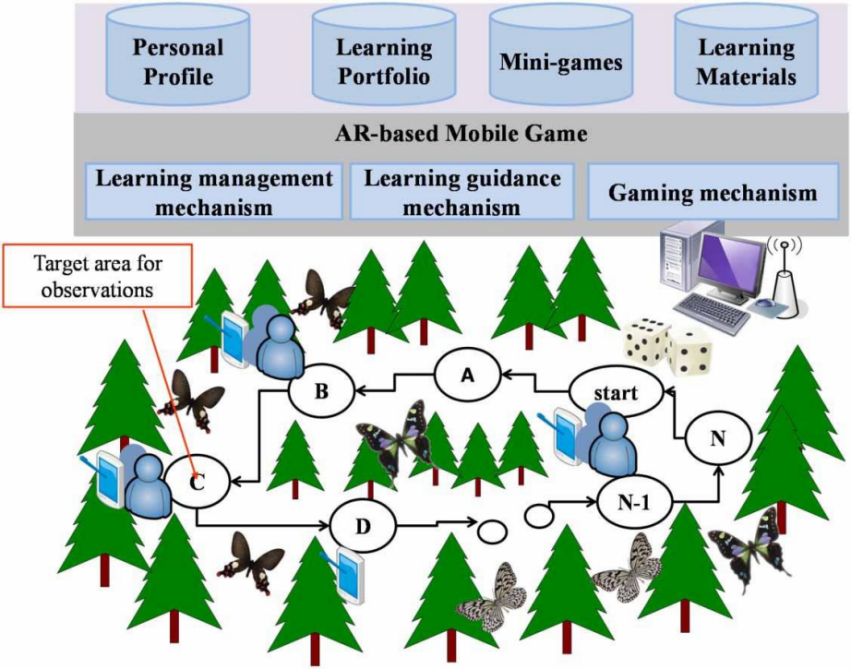
\includegraphics[scale=0.7]{figures/penelitian1.png}
    \caption{Augmented Reality Based Mobile Game System Structure.}
    \vspace{1em}
   \small Source: G.J. Hwang et al. (2016), Effects of an augmented reality-based educational game on students’ learning achievements and attitudes in real-world observations, \textit{Interactive Learning Environments}, pp. 4.
    \label{fig:my_label}
\end{figure}
This research has used a database to store assets and scenarios used. However, in this study, the application has not added 3D assets to present interactive learning so that it is more attractive to students' learning interests. This research has also not been applied to mobile devices with the iOS operating system so it can only be operated for Android OS, it also still uses QR code technology so it is necessary to develop a platform for markerless AR technology.

\begin{table}[h!]
\centering
\caption{Augmented Reality SDK Comparison. }
%\begin{adjustbox}{width=\columnwidth,center}
\resizebox{9cm}{!}{
\begin{tabular}{|c|c|c|c|c|c|c|c|c|c|} 
\toprule
\multicolumn{2}{|l|}{AR SDK}                                                          & \multirow{2}{*}{Vuvoria}                                                                  & \multirow{2}{*}{Metaio}                                                                          & \multirow{2}{*}{Wikitude}                                         & \multirow{2}{*}{ARToolkit}                                                              & \multirow{2}{*}{D'Fusion}                                                                & \multirow{2}{*}{ARmedia}                                          & \multirow{2}{*}{ARcore}                                                                                & \multirow{2}{*}{ARkit}                                           \\ 
\cline{1-2}
\multicolumn{2}{|c|}{Type}                                                            &                                                                                           &                                                                                                  &                                                                   &                                                                                         &                                                                                          &                                                                   &                                                                                                        &                                                                  \\ 
\hline
\multirow{6}{*}{Tracking} & Marker                                                    & \begin{tabular}[c]{@{}l@{}}Frame \\markers, \\image\\target, \\text \\target\end{tabular} & \begin{tabular}[c]{@{}l@{}}ID, \\picture \\and \\LLA \\marker, \\QR \\and \\Barcode\end{tabular} & \begin{tabular}[c]{@{}l@{}}Image,\\barcode\\tracking\end{tabular} & \begin{tabular}[c]{@{}l@{}}square \\marker, \\multiple \\marker \\tracking\end{tabular} & \begin{tabular}[c]{@{}l@{}}multiple\\marker,\\tracking,\\barcode \\tracking\end{tabular} & \begin{tabular}[c]{@{}l@{}}track \\fiducial \\marker\end{tabular} & \begin{tabular}[c]{@{}l@{}}motion\\tracking,\\build\\under-\\standing\\of the\\real world\end{tabular} & \begin{tabular}[c]{@{}l@{}}image,\\world\\tracking\end{tabular}  \\ 
\cline{2-10}
                          & GPS                                                       & N                                                                                         & Y                                                                                                & Y                                                                 & N                                                                                       & Y                                                                                        & Y                                                                 & Y                                                                                                      & Y                                                                \\ 
\cline{2-10}
                          & IMU                                                       & N                                                                                         & Y                                                                                                & Y                                                                 & N                                                                                       & Y                                                                                        & Y                                                                 & Y                                                                                                      & Y                                                                \\ 
\cline{2-10}
                          & Face                                                      & N                                                                                         & Y                                                                                                & N                                                                 & N                                                                                       & Y                                                                                        & N                                                                 & Y                                                                                                      & Y                                                                \\ 
\cline{2-10}
                          & \begin{tabular}[c]{@{}l@{}}Natural \\Feature\end{tabular} & Y                                                                                         & Y                                                                                                & Y                                                                 & Y                                                                                       & Y                                                                                        & Y                                                                 & Y                                                                                                      & Y                                                                \\ 
\cline{2-10}
                          & \begin{tabular}[c]{@{}l@{}}3D \\Object\end{tabular}       & Y                                                                                         & Y                                                                                                & N                                                                 & N                                                                                       & Y                                                                                        & Y                                                                 & Y                                                                                                      & Y                                                                \\
\bottomrule
\end{tabular}}
%\end{adjustbox}
\label{Tab:Table1}\\
\vspace{1em}
\small Source: Amin et al. (2015), Comparative  Study  of  Augmented  Reality  Sdk’s, \textit{International Journal on Computational Science}, pp. 25.
\end{table}

\begin{table}[h!]
\centering
\caption{Limitation AR SDK.}
\label{Tab:Table2}
\resizebox{7cm}{!}{
\begin{tabular}{|l|l|} 
\toprule
\multicolumn{2}{|l|}{Limitation}                                                                                                                                                                                              \\ 
\hline
Vuforia   & \begin{tabular}[c]{@{}l@{}}vuforia SDK for android doesn't expose any utility function \\to easily local a 3D model from any standart format. \\device database can only support 100 images targets\end{tabular}  \\ 
\hline
Metaio    & \begin{tabular}[c]{@{}l@{}}difficult to render complex 3D objects also limitation\\is associated with model size\end{tabular}                                                                                     \\ 
\hline
Wikitude  & \begin{tabular}[c]{@{}l@{}}doesn't track 3D model with limits is use to \\only 2D tracking. Target image to track need to \\be of solid colors to be recognizes\end{tabular}                                      \\ 
\hline
ARToolkit & \begin{tabular}[c]{@{}l@{}}less accuracy in tracking markers even when \\camera and marker are still. It itself doesn't \\support location based AR\end{tabular}                                                  \\ 
\hline
D'Fusion  & \begin{tabular}[c]{@{}l@{}}video file supported but audio associated\\with video can't be played\end{tabular}                                                                                                     \\ 
\hline
ARmedia   & doesn't support all type of textures for 3D objects                                                                                                                                                               \\ 
\hline
ARcore    & \begin{tabular}[c]{@{}l@{}}ARCore, on the other hand, will run on portable \\devices on a base of Android 7.0 Nougat and higher.\end{tabular}                                                                     \\ 
\hline
ARkit     & \begin{tabular}[c]{@{}l@{}}doesn't support android OS, need depth camera. \\ARKit is only compatible with iPads or \\iPhones on a base of iOS 11 and higher.\end{tabular}                                         \\ \hline
\end{tabular}}\\ 
{\vspace{1em}}
\small Source: Amin et al. (2015), Comparative  Study  of  Augmented  Reality  Sdk’s, \textit{International Journal on Computational Science}, halaman 23.
\end{table}


